\documentclass[border=2mm,tikz]{standalone}
\usepackage{tikz}
\usetikzlibrary{datavisualization}
\usetikzlibrary{datavisualization.formats.functions}
\begin{document}
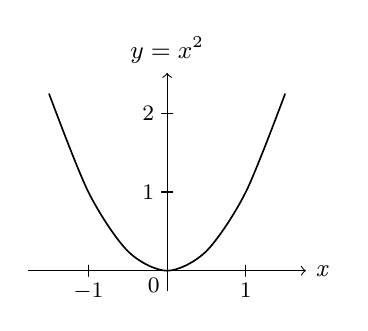
\begin{tikzpicture}
\datavisualization [school book axes,
                    visualize as smooth line,
                    y axis={label={$y=x^2$}},
                    x axis={label} ]

data [format=function] {
      var x : interval [-1.5:1.5] samples 7;
      func y = \value x*\value x;
      };
\end{tikzpicture}

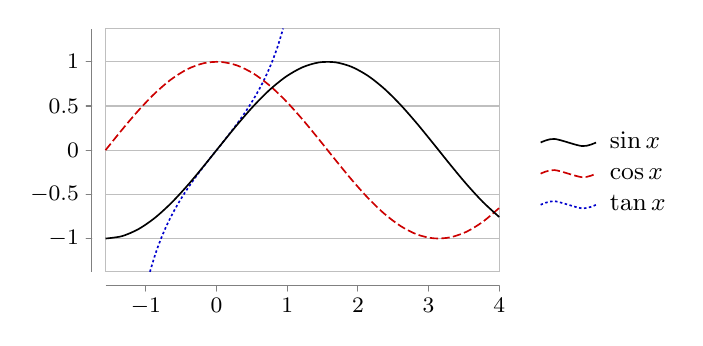
\begin{tikzpicture}
\datavisualization [scientific axes=clean,
                    y axis=grid,
                    visualize as smooth line/.list={sin,cos,tan},
                    style sheet=strong colors,
                    style sheet=vary dashing,
                    sin={label in legend={text=$\sin x$}},
                    cos={label in legend={text=$\cos x$}},
                    tan={label in legend={text=$\tan x$}},
                    data/format=function
                    ]
data [set=sin] {
  var x : interval [-0.5*pi:4];
  func y = sin(\value x r);
}
data [set=cos] {
  var x : interval [-0.5*pi:4];
  func y = cos(\value x r);
}
data [set=tan] {
  var x : interval [-0.3*pi:.3*pi];
  func y = tan(\value x r);
};
\end{tikzpicture}
\end{document}